%In addition you need a substantial (10-20 pages) introductory chapter detailing
%  Significance (Why was the research done needed) and
%  Innovation (Why was the research done novel? How does it relate to competing methods?) of the body of work in your thesis.
%This chapter could ideally come form a review article you have written.
\chapter{Introduction}
\label{chap:chapter1}
\section{Antibody Overview}
The lymphocytes that make up the adaptive immune system have evolved to recognize a limitless number of antigens that constitute viruses, bacteria and all foreign material to a hosts immune system  \citep{Murphy:2007tl}. The concern of this thesis is on the antigen-recognition molecules of the B-cell known as immunoglobulins (Ig). These can exists either as a membrane-anchored form to the B-cell known as the B-cell receptor (BCR) or as a secreted form with a wide range of functionality known as the antibody. The main effector function of the antibody is to bind foreign pathogens in the body and is the basis for the adaptive immune response. The antibody molecule has two separate functions. One is to bind specifically to molecules known as antigens. The other is to recruit other cells and molecules to destroy the pathogens each immunoglobulin is bound to. There are two genetic domains that make up the antibody structure and differentiate these processes (figure \ref{fig:antibodyoverview}). One is the variable domain responsible for specificity. The other is the constant domain that engages different effector functions such as cytokine recruitment and phagocytosis of compromised cells. Structurally, antibodies consist of two identical heavy chains, that are recombined gene segments of the heavy variable and constant domain gene segments, and two identical light chains, which are recombined copies of light chain variable and constant domains gene segments.

The variability of the antibody molecule is what ensures that any individual with a functional immune system can produce an antibody to recognize almost any structure. The mechanisms of variability are discussed in further sections but are typically distributed to the apical tips of the antibody structure. It is important to note that the B-cell bound receptor and effector function of antibodies play an important role in the humoral immune system, but the remainder of this document will focus on the diversity and specificity of secreted antibodies of the IgG class, the most common circulating immunoglobulin.  

\begin{figure}%Antibody Structure
\centering
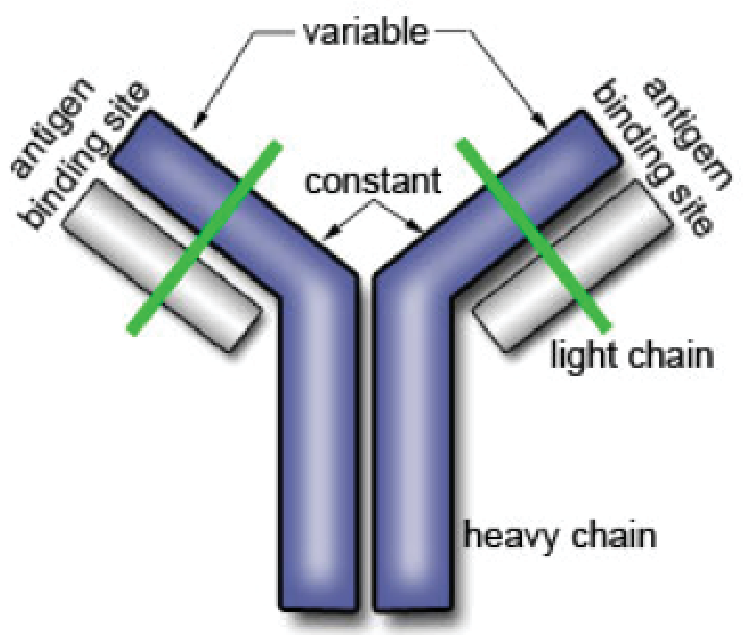
\includegraphics[width=.45\textwidth]{images/intro/figure1_1.pdf}
\caption[Overview of Antibody Structure]{
Overview of Antibody Structure. Heavy chain is shown in blue, light chain in grey. The structure is divided into the variable portion responsible for recognition, and the constant portion responsible for effector function. The apical tips of the antibodies are where antigens typically bind and are therefore known as the antigen binding sites. Image reproduced from http://crdd.osdd.net/raghava/absource/abasic.html.
}
\label{fig:antibodyoverview}
\end{figure}

\subsection{Antibody Diversification}
The antibody genes that encode heavy and light chains are located in three primary locations in the human genome: heavy chain genes (IGH) are located on chromosome 14, light chain kappa genes (IGK) are located on chromosome 2, and light chain lambda genes (IGK) are located on chromosome 22 \citep{Brochet:2008kq}. Each of these loci consists of multiple variable (V, not to be confused with the variable region of an antibody) and joining (J) gene segments. In addition the IGH locus also contains several diversity (D) gene segments.  Sequencing of the human IGH locus revealed 55 functional V genes, 23 D genes, and six J genes \citep{Matsuda:1998ua,Lefranc:2009ga}. The human variable genes (and, at the IGH locus, the diversity genes) can be phylogenetically grouped into families based on sequence similarity. Heavy chain variable genes are organized into seven families and homology within gene families is typically above 80\%. The 23 functional human diversity genes are also organized into seven families. An example variable gene, IGVH5-15*01, the standard IMGT nomenclature for human V and D genes follows the following pattern: the chain and gene description (IGHV for variable genes, IGHD for germline genes), the family, the gene number (determined by position in the germline locus), and the allele. The gene number is separated from the family with a hyphen and the allele is separated from the gene number with an asterisk.


\subsubsection{Recombination to Enable Diversity}
The tremendous sequence and structural diversity  can be attributed to two immunologic processes that act on antibody germline gene segments. The first is the initial recombination initiated by the recombination activating gene machinery (RAG) \citep{Brack:1978ie,Alt:1982uq,Tonegawa:1983vw,Schatz:1989tk,Oettinger:1990ud}. The RAG machinery is responsible for the recombination of V, D, and J gene for the heavy chain, and the V and J gene for the light chain (figure \ref{fig:Diversification}, left-panel). This process takes place to make functional B-cell receptors in the bone marrow before antigenic stimuli. If a B-cell receptor is found to bind self-antigens of the host, it is eliminated. This clonal selection and deletion is the fundamental process for which antibodies are able to recognize foreign antigens while not attacking the host.
 
Much progress has been made in determining the genetic and mechanistic elements that participate in the antibody recombination process. Recombination signal sequences (RSS), which flank V, D and J genes and are composed of conserved AT-rich heptamer and nonamer sequences separated by spacers of either 12 or 23 nucleotides, are recognized and bound by recombination activating gene (RAG1 and RAG2) proteins at the initiation of the recombination process \citep{Hesse:1989us,Alt:1992bh}. Recombination typically occurs only between RSS elements of different spacer lengths, in a model commonly referred to as the 12/23 rule of recombination \citep{Ramsden:1996tw,Steen:1996ut,vanGent:1996uw,Schatz:2011hb}. After binding to one 12-bp RSS and one 23-bp RSS, the RAG complex induces single-strand DNA nicks between the coding sequence and the heptamer of each RSS, resulting in hairpin formation on each of the coding ends and a blunt double-stranded break on each signal end \citep{Roth:1992wg,Schlissel:1993tg,McBlane:1995kp,Sadofsky:2001we}. The hairpins are opened with other RAG mutation machinery (Artemis) \citep{Ma:2002en}.  Nucleotides may be added to or removed from the coding ends, and the double strand breaks at the coding ends are joined into a single coding strand with DNA ligase IV \citep{Lewis:1994vp,Mahajan:1999wz,Shockett:1999vp,Walker:2001kn,MansillaSoto:2003ws,Roth:2003ji} (figure \ref{fig:Diversification}, middle panel). The newly recombined gene produces a functional antibody (figure /ref{fig:Diversification}, right panel). Recombination of the light chain is similar but the result of a single V$_{L}$J$_{L}$ recombination. To establish a diverse na�ve antibody repertoire, these events of RAG-mediated recombination produce an initial repertoire of ~3x10$^{7}$ different recombinations. This happens all before antigen stimulus in the bone marrow leading to the next form of antibody diversity, somatic hypermutation.

\begin{figure}%Recombination Diversification
\centering
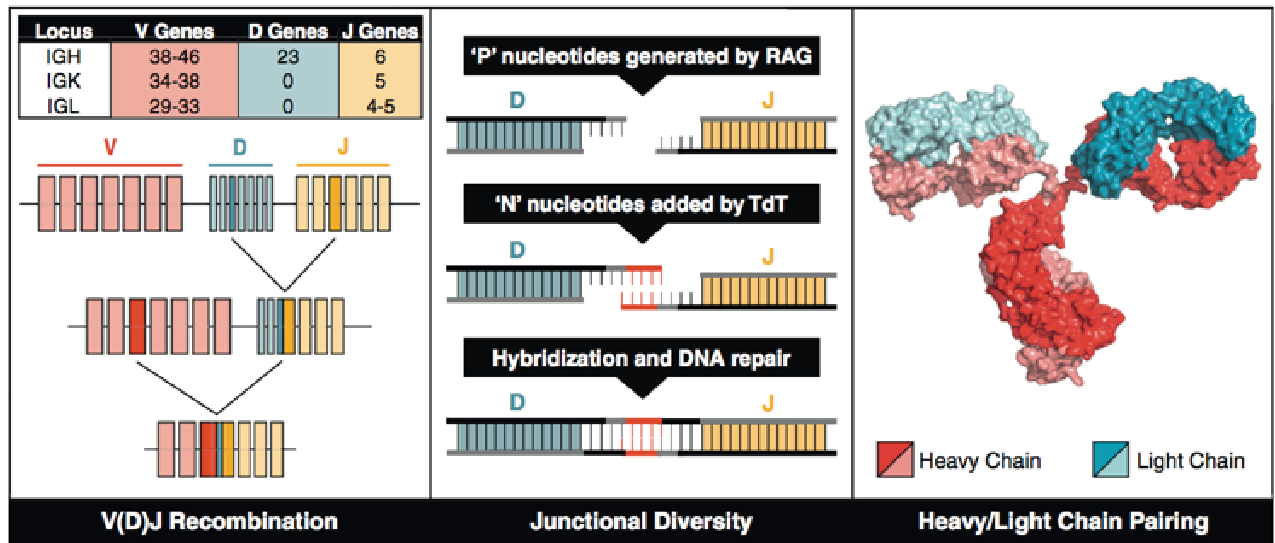
\includegraphics[width=1\textwidth]{images/intro/figure1_2.pdf}
\caption[Overview of Antibody Recombination]{
Overview of Antibody Recombination. Diversity in the antigen-combining site of the B-cell receptor repertoire (and thus also in the corresponding secreted antibody repertoire) is mediated by three principal molecular mechanisms, illustrated in the three panels, left, middle, and right. Figure adapted from \citep{Finn:2013fr}.
}
\label{fig:Diversification}
\end{figure}


\subsubsection{Somatic Hypermutation to Enable Diversity}
Maturation of the antibody repertoire to hone specificity is known as somatic hypermutation (SHM) and is initiated by the somatic hypermutation machinery (SHAM). Somatic hypermutation is the response to antigen stimulus and happens in various lymph tissues. This process is known as the secondary diversification \citep{Tonegawa:1983vw,Brenner:1966vj}. 

Na�ve, antigen inexperienced B-cells undergo the SHM process upon recognition of an infectious agent. It is through the SHM process, which occurs primarily in lymphoid tissue, mutate the variable region of their antibody genes (figure \ref{fig:somaticdiversification})  \citep{Li:2004it,MacLennan:1992we}. Many of these mutations have no effect on antigen recognition and many have deleterious effects on either antigen recognition or proper folding of the antibody protein. However, some mutations produce antibodies with improved affinity for the target pathogenic epitope  \citep{Casali:2006dn}.Thus, the SHM process provides a basis for the positive selection of high affinity antibodies that are characteristic of a mature immune response  \citep{MacLennan:1994bo}. SHM introduces point mutations at a frequency of approximately 103 mutations per base pair, which is 106-fold higher than the rate of spontaneous mutation in other genes \citep{Rajewsky:1987wn}. Activation-induced cytidine deaminase (AID) is required for SHM and initiates the SHM process by the deamination of cytosine nucleotides, which results in the conversion of cytosine to uracil \citep{Muramatsu:2000um,Muramatsu:1999ur}. Deamination thus produces a uracil-guanine mismatch, and several possible processes result in the error-prone repair of the mismatch. The precise mechanism(s) responsible for error-prone repair during SHM are not known, although several DNA repair mechanisms have been shown to be critical to the SHM process, including base excision repair and mismatch repair \citep{Phung:1998vx,Rada:1998tf,Wiesendanger:2000wl,DiNoia:2002ix,Zheng:2005dy}. 

\begin{figure}%Somatic Diversification
\centering
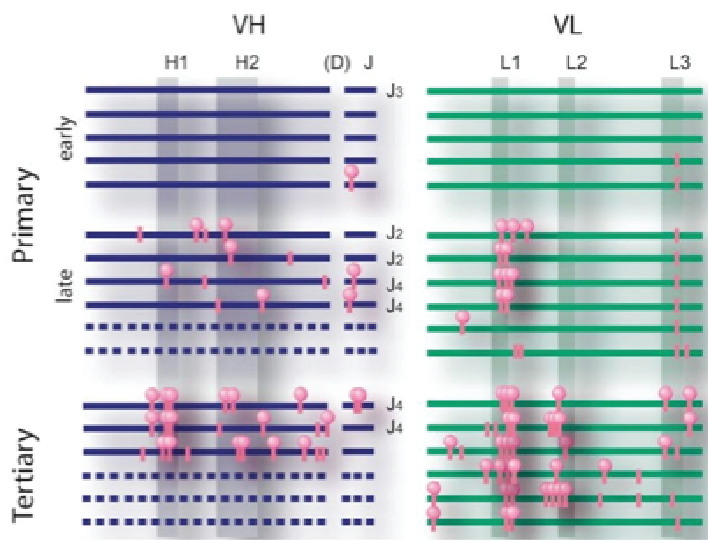
\includegraphics[width=.5\textwidth]{images/intro/figure1_3.pdf}
\caption[Somatic Mutations in Response to Antigen Stimulus]{
Somatic mutations in response to antigen stimulus. The VH gene and VL gene are shown for various VH and VL pairs represented by blue and green lines. The CDR loops H1-H3 and L1-L3 are darkened. The pink dots represent mutations. The early response has little to no somatic mutations recapitulating na�ve repertoire. The late and response starts developing mutations. A second challenge with the same antigen shows even more mutations to hone specificity. Figure adapted from \citep{Berek:1988ww}, redrawn by C., Scotti. }
\label{fig:somaticdiversification}
\end{figure}

\subsubsection{Implications for Antibody Structure}
Antibody complementarity determining regions (CDRs, also referred to as hypervariable regions, figure /ref{fig:abwithloops}) are the primary region of antigen recognition that lie at the apical tip of the antibody structure (figure \ref{fig:abwithloops}). They are preferentially targeted for affinity maturation by the SHM machinery, making them the most variable regions of the antibody gene \citep{Padlan:1994wq}.  Structurally, the CDRs are largely loop-based, which make them sufficiently flexible to incorporate the substitutions and without compromising structural integrity. Framework regions (FRs) are highly structured and less able to accommodate somatic mutations \citep{Jimenez:2003by}.

\begin{figure}%Antibody with Loops
\centering
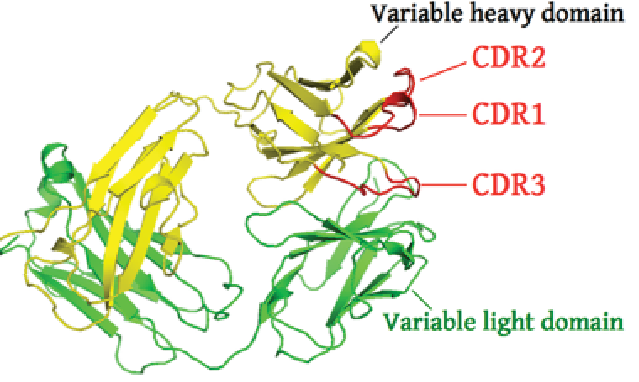
\includegraphics[width=.5\textwidth]{images/intro/figure1_4.pdf}
\caption[Antibody Structure with CDR Loops]{Antibody structure with CDRs.The light chain in green with the LCDRs not pictured. The heavy chain is shown in yellow with the HCDRs shown in red. Figure adapted from PDB: 1IGT\citep{Harris:1997eo}.
}
\label{fig:abwithloops}
\end{figure}

\section{HIV Pandemic Overview}
HIV-1 is an unprecedented health problem that continues to remain a worldwide pandemic. Since the recognition of acquired immune deficiency syndrome (AIDS) in 1981 \citep{Gottlieb:1981ge} followed by the discovery of it's causative agent, human immunodeficiency virus (HIV) in 1983 \citep{BarreSinoussi:1983ta}, an estimated 65 million have been infected with over 25 million deaths \citep{Hemelaar:2012cv}. The amount of people estimated to be still living with HIV is 30 million, many of which live in the developing world \citep{Anonymous:1vVbBZBX}.

More than 40 different nonhuman primate species harbor SIV infections, with each species carrying a species-specific virus. Each independent zoonotic transmission can generate a different lineage. HIV type 1 (HIV-1), thought to be transmitted from chimpanzees in the Congo around 1900 \citep{Keele:2006fi}, is the most common and further is split into groups M, N, O, and P. HIV-1 group M is responsible for the global pandemic and is further split into subtypes clades A-D,F-H, J and K that are tropic to specific regions. Within each subtype variation of the amino acids vary as much as 30\%. For example, clade B is the most common in North America while clade C is the most common in Sub-Saharan Africa (figure \ref{fig:pandemic}). If a full genome sequence is found that are recombinations of different HIV-1 group M subtypes, they are designated circulating recombinant forms (CRFs) if they are epidemiologically linked or unique recombinant forms if they are unlinked (URF) \citep{Robertson:2000bv}.

A major contributing factor to HIV spread and defense is its potential for enormous genetic diversity. This genetic diversity stems from the error rates of the reverse-transcription machinery which lacks proof-reading capabilities \citep{Ho:1995fn}. This genetic diversity gives rise to sequence divergence of up to 10\% within a single individual \citep{Korber:2001tc}. This is one of the many defense mechanisms HIV uses to evade host response and contemporary vaccination strategies.

\begin{figure}%HIV Pandemic
\centering
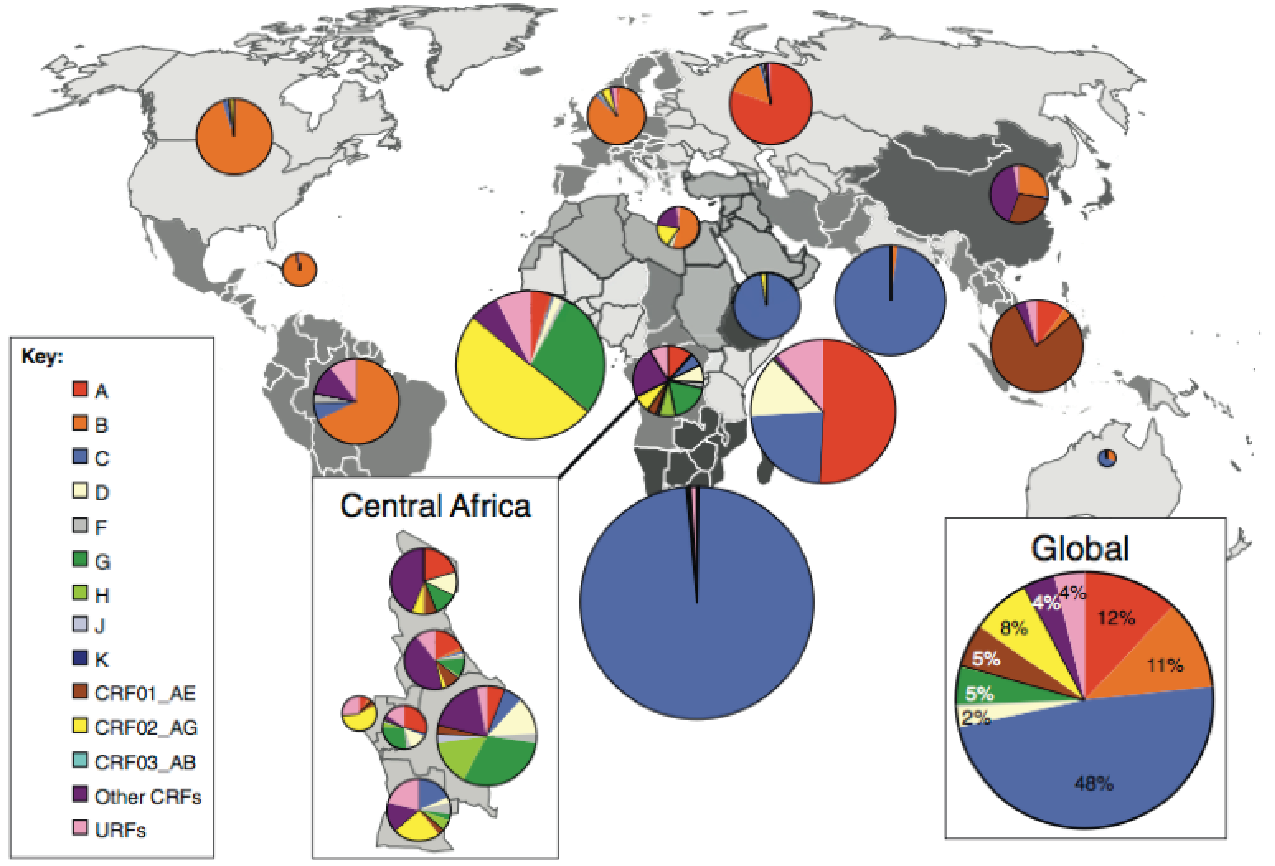
\includegraphics[width=1\textwidth]{images/intro/figure1_5.pdf}
\caption[Global Distributions of HIV-1 Subtypes]{Global distributions of HIV-1 subtypes. In the main figure, pie charts representing the distribution of HIV-1 subtypes and recombinants from 2004 to 2007, colored by HIV-1 subtype. Adapted from UNAIDS report 2013.}.
\label{fig:pandemic}
\end{figure}

\subsection{The HIV Virus Genome and Structure}
HIV-1 is an enveloped virus containing a duplicate positive-strand RNA genome (figure \ref{fig:hivgenome}, left panel). The functional spike on the surface of the virion is the Env glycoprotein and is coded by the env gene (figure \ref{fig:hivgenome}, right panel). The Env glycoprotein complex is originally produced as a single-chain glycoprotein precursor, gp160, which is cleaved by a cellular protease. Cleavage of gp160 results in the cell-surface attachment protein gp120 and the membrane-spanning protein gp41. The gp160 cleavage products are noncovalently linked and assemble into a trimer of gp120-gp41 heterodimers that are expressed on the virion surface \citep{Kowalski:1987vq}. Gp120 is heavily glycosylated, with nearly half the total mass being the result of N-linked glycans \citep{Poignard:2001hu}. It is composed of five variable regions (V1-V5) interspersed with five constant regions (C1-C5) \citep{Starcich:1986ty}. The principle function of the glycoprotein spike is to facilitate cell entry by binding to the primary cell-surface receptor, CD4, and one of the two co-receptors, CCR5 and CXCR4. Binding to the receptor and co-receptor is accomplished by gp120, and fusion of the viral and cell membranes is mediated by gp41 \citep{Zwick:2001ei}. 

The rest of the genome is composed of viral enzymes such as the error-prone reverse transcriptase, the integrase that allows integration of viral DNA to the host genome, and protease, to allow cleavage of gene products into their functional subunits. There are also structural proteins that lie below the envelope that make up the inner matrix and nucleocapsid. There are also several accessory proteins, Vpu, Vif, Vpr, P6, Nef, Rev, and Tat which aid in combating host defense or enhancing viral fitness \citep{Fields:2007vu}. All of these proteins serve a significant purpose to the virulence and life cycle of the HIV-1 virus but will not be discussed further and they have low antigenicity to antibodies, the primary focus of my research. A list of their genes and gene products can be found in figure \ref{fig:hivgenome}, right panel. 

\begin{figure}%HIV Genome and Structure
\centering
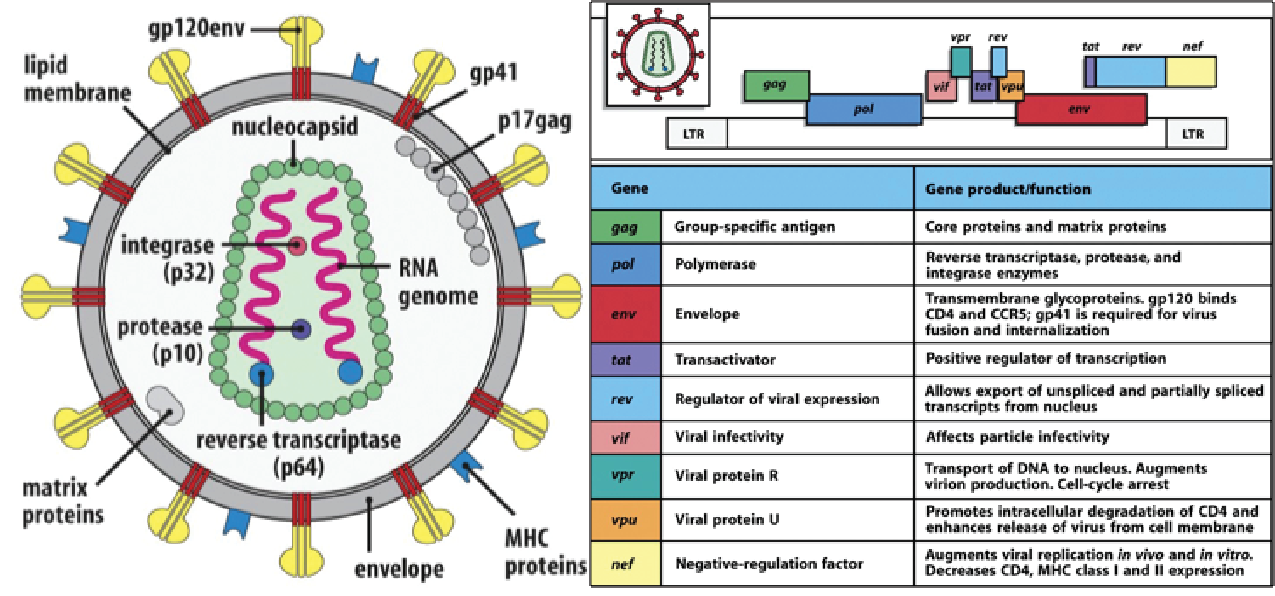
\includegraphics[width=1\textwidth]{images/intro/figure1_6.pdf}
\caption[Simplified View of HIV Structure and Genome]{Simplified view of HIV structure and genome. The proteins that make up the virus structure are displayed as a schematic. The virus is coded by a duplicated RNA genome (pink) surrounding by a viral nucleocapsid proteins. The inner envelope is supported by gag protein with gp120 envelope shown as a trimer bound to gp41. These trimeric "spikes" are responsible for infectivity by binding CD4-binding sites (left panel).\linebreak Each gene is represented in a different color and localizes to either the nucleocapsid (green) or the outer envelope (red). }
\label{fig:hivgenome}
\end{figure}

\subsection{The Viral Spike and Humoral Resistance}
The failure of conventional vaccines to prime the immune system for a broad response against HIV-1 challenge is partially explained thorough the structural definition of the HIV-1 spike reveling mechanisms of defense. Much of the surface is covered in carbohydrates that shield neutralizing epitopes \citep{Binley:2010du}. The conserved CD4 binding site is recessed and sits behind the hypervariable loops \citep{Burton:2005db}. The co-receptor binding site is also recessed unless CD4 has triggered a conformational shift exposing this region \citep{Harris:2011gm}. Another defense is the relative lability of the trimeric complex \citep{Wyatt:1998vs}. The gp120 head often sheds creating "stumps" that serve as decoy epitopes against the viral complex \citep{Liu:2008in}. In addition there are few functional trimeric spikes on the surface of HIV limiting immune response to few locations on the virion. 

The biggest defense is sequence variability. Much of the antibody response is targeted to the hypervariable loops that can easily change sequence without much consequence to viral fitness. This is why the humoral response produces autologous or strain-specific neutralizers that must catch up to a constantly evolving antigenic target \citep{Albert:1990ua,Gray:2007hi,Pilgrim:1997wj,Richman:2003dc,Sagar:2006eb,Wei:2003ea}.  

\section{Broadly Neutralizing Antibodies to HIV}
Given the major defenses of the HIV envelope structure, it provided a rather discouraging view for vaccine development. In fact, only four modestly neutralizing antibodies were discovered between the 1991 and 2010 \citep{Burton:2005db,Kwong:2012cc}, two membrane proximal extracellular region (MPER) binders 2F5 and 4E10 \citep{Zwick:2001ei,Muster:1994tw}, a CD4 binding site neutralizer b12 \citep{Burton:1994wl}, a complex carbohydrate binder 2G12 \citep{Trkola:1996vb} (table \ref{tab:allmabs}, figure \ref{fig:bnabmap}). 

It was thought that the conventional vaccine strategies could not stimulate immune system to produce broadly neutralizing antibodies to HIV do to the extreme variability of the viruses and the capability of the virus to escape an antibody response. Then, high throughput neutralization assays were developed that could rapidly test sera for neutralization capacity \textit{in vitro} allowing researchers to accurately quantify the neutralizing response of HIV infected patients \citep{Binley:2004hd,Blish:2007ef,Li:2005go,Mascola:2005fe,Montefiori:2005jt}. Several groups found that there were multiple patients that could neutralize very genetically diverse panels HIV variants, even those that were not in that patients sub-type \citep{Binley:2008gj,DoriaRose:2010js,Simek:2009cn,Wu:2006cd}. That lead to longitudinal studies to show how long it took for a broadly neutralizing response to develop. Researchers showed that this generally took anywhere from 2-4 years \citep{Gray:2011ki,Mikell:2011hr,Moore:2011hy} with earliest time points arising at 1 year \citep{DoriaRose:2014ic}. The question still remained if those neutralizing responses were caused by few monoclonal antibody responses or just a large polyclonal response \citep{Gray:2007hi,Binley:2008gj,Li:2007em,Rong:2009ky,Sather:2009jb,Scheid:2009bv,Tomaras:2011bc,Walker:2010bm}.

The question was answered by the recent explosion of new broadly neutralizing antibodies isolated by multiple research groups \citep{Corti:2013ex}. It started with two new isolates, PG9 and PG16, from an African donor that lead to the discovery of a completely new neutralizing epitope which is the focus of my research (figure  \ref{fig:bnabmap}) \citep{Walker:2009cd}. Both PG9 and PG16 bind to a proteoglycan epitope through an extended HCDR3 structure \citep{McLellan:2011dg}. 

The discovery of PG9 and PG16 lead to newly characterized antibodies using similar techniques such as microneutralization screening, high-throughput sequencing, and hybridoma technology. The Haynes laboratory characterized additional long HCDR3 antibodies that bound similarly as PG9 and PG16 but with less breadth \citep{Bonsignori:2011dq}. There are other classes of glycan dependent antibodies isolated by the Poignard group that bind the V3 and beta-strands that are higher potency than PG9 and PG16 \citep{Walker:2011ew}. Other MPER antibodies have also been characterized to by the Connors group such as 1E08 that neutralizes 98\% of viruses \citep{Huang:2012fh}. Focused epitopes designed computationally can also be used to identity some of the most potent antibodies to date (the VRC series) \citep{Wu:2010jv}. These antibodies were identified using a designed scaffold of gp120 that 'knocked-out' non-neutralizing epitopes. Thus, only neutralizing antibodies would be isolated upon binding. I will not enumerate further on all the antibodies characterized to date, their method of isolation and if any longitudinal studies were used to determine their pathways of development. These characteristics are summed in table \ref{tab:allmabs} and figure \ref{fig:bnabmap}.

It is interesting to note, and important for the work that will be presented here, that the broadly neutralizing antibodies to date share one of two characteristics. They are either highly somatically mutated, indicative of years of chronic infection and selective pressure, or have a very long non-canonical HCDR3 (figure \ref{fig:bnabcorrelation}). Both of these characteristics make it difficult to elicit in a vaccine attempt, but will be discussed further in the upcoming chapters.

%comes from excel to table
% Table generated by Excel2LaTeX from sheet 'page 1'
\begin{sidewaystable}[htbp]
  \centering
\begin{tabular}{lllllcl}
\toprule
Antibody & Specificity & Breadth & V$_{H}$ & SHM & HCDR3 Length & Screening Strategy \\ 
\midrule
	2F5 & gp41 MPER & \textasciitilde60-70\% & 2-5 & 15.2 & 24 & gp160 and p24 binding \\
	4E10 & gp41 MPER & \textasciitilde96-98\% & 1-69 & 15.6 & 20 & gp160 and p24 binding   \\ 
	1EO8 & gp41 MPER & \textasciitilde98\% & 3-15 & 22.1 & 22 & Microneutralization  \\ 
	2G12 & gp120 glycans & \textasciitilde25-30\% & 3-21 & 33.6 & 16 & gp160 and p24 binding   \\ 
	PGT128 & Glycans and V3 $\beta$-strand & \textasciitilde70-75\% & 4-39 & 27.9 & 21 & Microneutralization  \\ 
	PGT127 & Glycans and V3 $\beta$-strand & \textasciitilde50\% & 4-39 & 23.2 & 21 & Microneutralization   \\ 
	PGT121 & Complex type V3 N-glycans & \textasciitilde65-70\% & 4-59 & 21.2 & 26 & Microneutralization  \\ 
	10-1074 & Complex type V3 N-glycans & \textasciitilde55-60\% & 4-59 & 24.4 & 26 & gp140 binding   \\ 
	PGT135 & Glycans and V4 & \textasciitilde30-35\% & 4-39 & 26.8 & 20 & Microneutralization   \\ 
	PG9/PG16 & Glycans and V1/V2 & \textasciitilde75-80\% & 3-33 & 15.4-16.8 & 30 & Microneutralization   \\ 
	CH01- CH04 & Glycans and V1/V2 & \textasciitilde50\% & 3-20 & 23.3-19.5 & 26 & Microneutralization  \\
	PGT145 & Glycans and V1/V2 & \textasciitilde75-80\% & 1-8 & 22.8 & 33 & Microneutralization \\
	b12 & gp120 CD4bs & \textasciitilde30-35\% & 1-3 & 17.3 & 20 & Phage library  \\ 
	HJ16 & gp120 CD4bs & \textasciitilde30-35\% & 3-30 & 36.7 & 21 & EBV- immortalization  \\ 
	VRC01 & gp120 CD4bs & \textasciitilde90-95\% & 1-2 & 38.7 & 14 & Cell sorting/RT-PCR \\
	VRC03 & gp120 CD4bs & \textasciitilde50\% & 1-2 & 34.9 & 16 & Cell sorting/RT-PCR \\ 
	3BNC117 & gp120 CD4bs & \textasciitilde85-90\% & 1-2 & 36.9 & 12 & Cell sorting/RT-PCR  \\ 
	3BNC60 & gp120 CD4bs & NA & 1-2 & 36.9 & 12 & Cell sorting/RT-PCR \\
	NIH45-46 & gp120 CD4bs & \textasciitilde90\% & 1-2 & 44 & 18 & Cell sorting/RT-PCR \\
	CH30- CH34 & gp120 CD4bs & \textasciitilde80\% & 1-2 & 31.9-31.9 & 15 & Cell sorting/RT-PCR  \\
	PGV04 & gp120 CD4bs & \textasciitilde85-90\% & 1-2 & 38.2 & 16 & Cell sorting/RT-PCR\\
	3BC176 & CD4i/V3 & \textasciitilde60-70\% & 1-2 & 29.4 & 19 & Cell sorting/RT-PCR \\
\bottomrule
\end{tabular}
\caption[Broadly Neutralizing Antibody Properties]{Broadly neutralizing antibody properties. Breadth refers to the amount of viruses tested that fall below 50 $\mu$g/mL.  V$_{H}$ is the heavy chain accessed from IMGT, SHM is the somatic hypermutation percentage of heavy chains as assessed from IMGT. Table adapted from (2013)\citep{Corti:2013ex}. }
\label{tab:allmabs}%
\end{sidewaystable}%


\begin{figure}[!t]%HIV man map
\centering
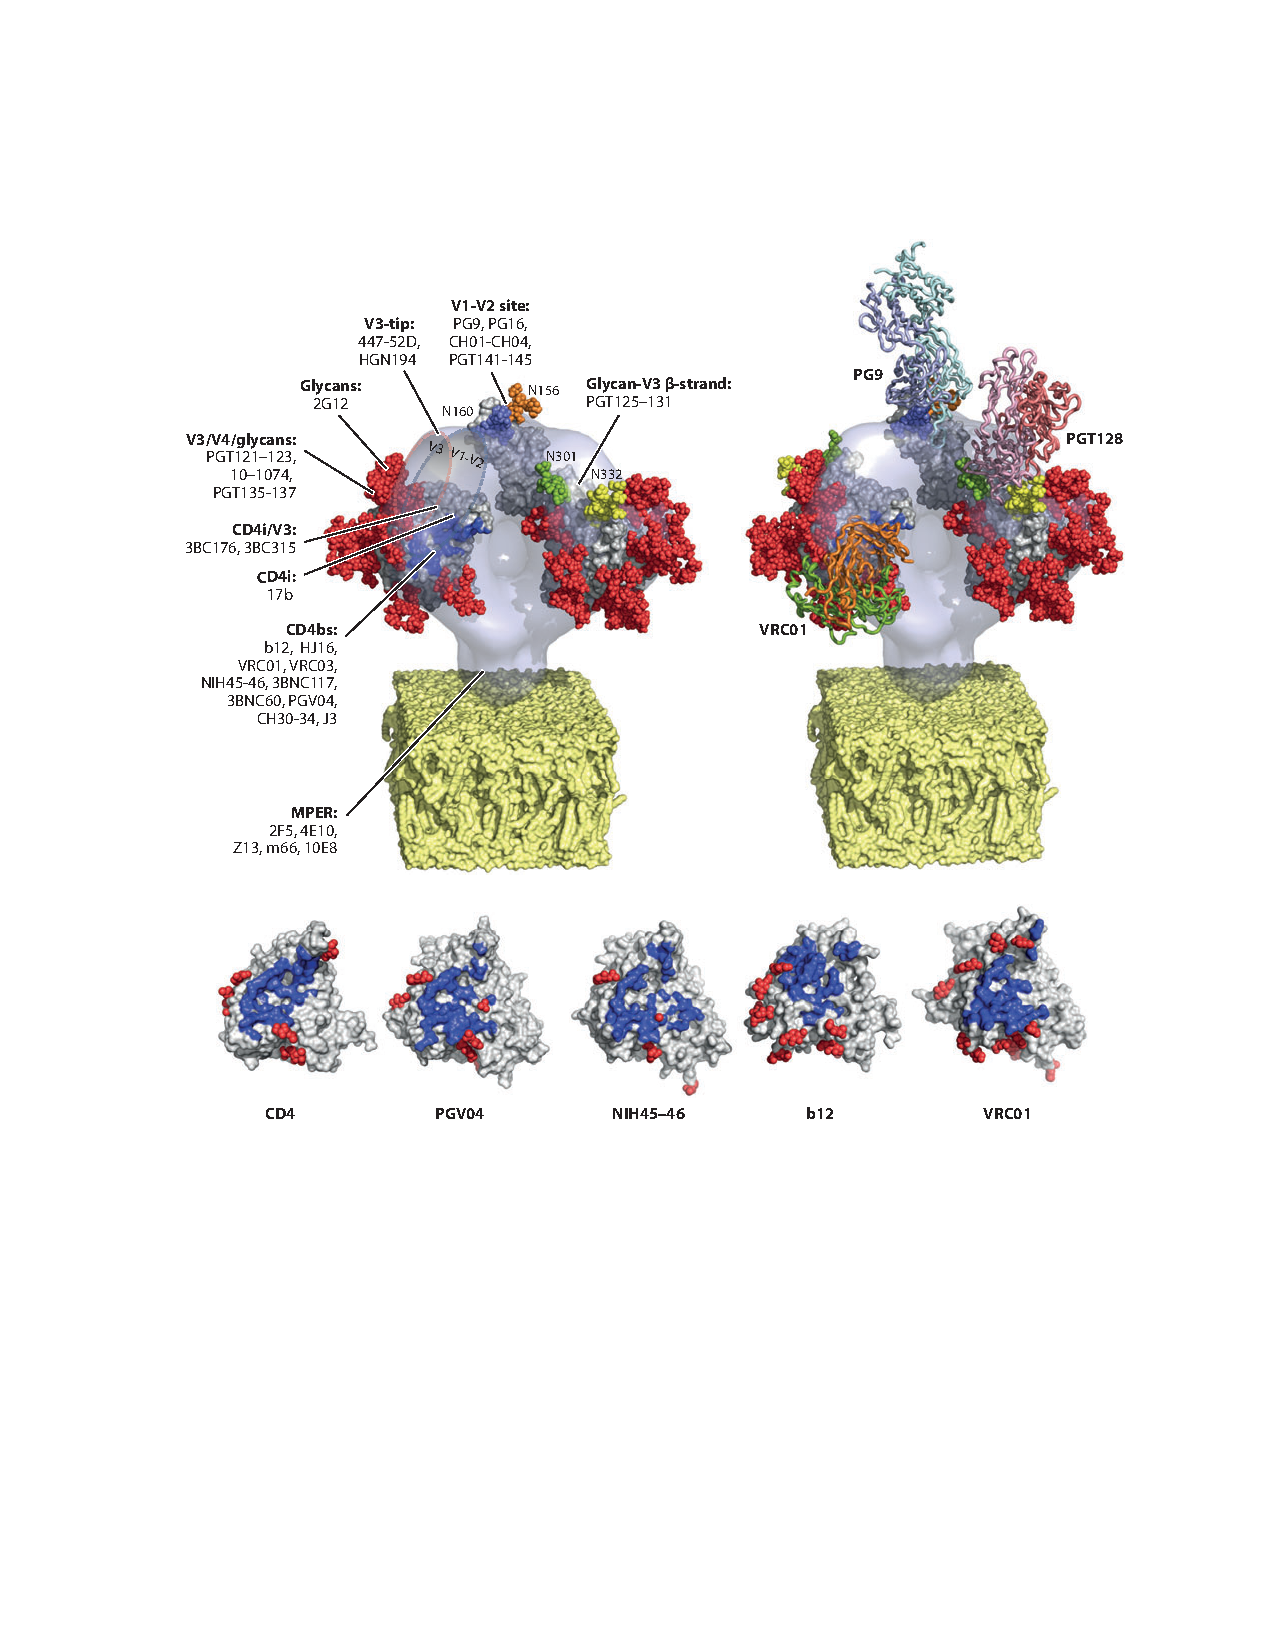
\includegraphics[width=1\textwidth]{images/intro/figure1_7.pdf}
\caption[Broadly Neutralizing Epitopes Mapped to HIV Env Trimer]{Model of the HIV-1 Env trimeric glycoprotein bound to broadly neutralizing antibodies. The left panel shows the major sites targeted by broadly neutralizing antibodies. The approximate positioning of the V1/V2 and V3 loops is shown, and the CD4 footprint on the gp120 monomer is highlighted in blue. The right panel shows the FABs of broadly neutralizing antibodies VRC01 (3NGB), PG9 (3US2), and PGT128 (3TYG) bound to gp120. Carbohydrates (oligomannose, red spheres) were modeled on the unliganded YU2 gp120 core (3TGQ) using GlyProt, with the exception of the glycans bound by PGT128 and PG9 (depicted with different colors), which were taken from the structures. The location of PG9 above the trimeric gp120 is approximate; VRC01 and PGT128 FABS were docked by superposition with the unliganded YU2 gp120 model. The bottom panel shows in blue the footprints of CD4 (1GC1) and the CD4bs-specific antibodies PGV04 (3SE9), NIH45-46 (3U7Y), b12 (3DNL), and VRC01 (3NGB). Figure adapted from \citep{Corti:2013ex}}
\label{fig:bnabmap}
\end{figure}

\begin{figure}%HIV man map
\centering
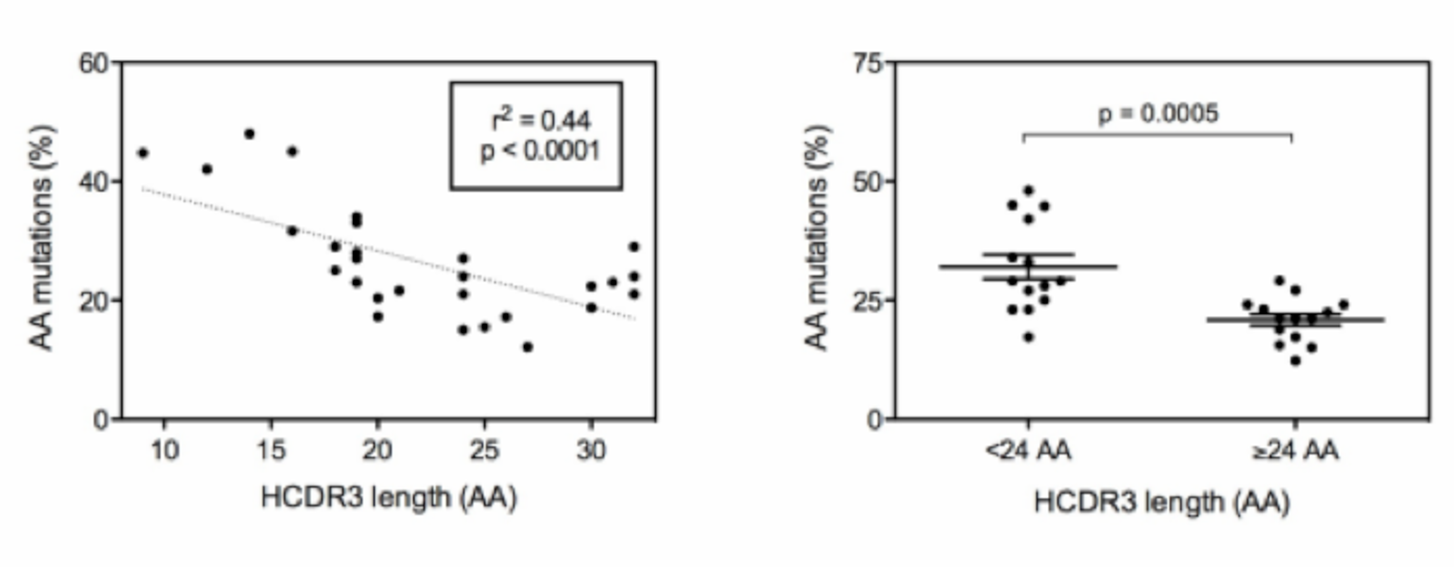
\includegraphics[width=1\textwidth]{images/intro/figure1_8.pdf}
\caption[Trends of HIV bNAbs]{Trends of HIV bNAbs. Plotted on the y-axis is the frequency of amino acid mutations of the currently characterized bNAbs. On the x-axis is the length of the heavy chain CDR3 (HCDR3). A negative correlation exists between the frequency of mutations and the HCDR3 length (r$^{2}$ = 0.44, left panel). When long HCDR3s (>24 AA) are binned against canonical length HCDR3s (<24AA), there is a statistical significance between the frequencies of amino acid mutation (p = 0.0005, right panel).}
\label{fig:bnabcorrelation}
\end{figure}



\section{Rosetta}
Many software packages exist for the specific task of threading, minimization, and design. The Rosetta software suite includes algorithms for all of these tasks and was developed for computational modeling and analysis of protein structures; further, it is free for noncommercial users. It has enabled notable scientific advances in computational biology, including de novo protein design, enzyme design, ligand docking and structure prediction of biological macromolecules and macromolecular complexes \citep{Rohl:2004bl,Siegel:2010bc,Kuhlman:2003kp,Davis:2009bf,Misura:2006hs,Davis:2009fx,Das:2008gf}. The broad spectrum of applications available through Rosetta allows for multiple computational problems to be addressed in one software framework. To aid in the understanding of Rosetta-specific language, a supplementary glossary has been provided in the appendix section for the Rosetta glossary.
One of the most common applications of Rosetta is protein structure prediction via \textit{de novo} folding and comparative modeling \citep{Kaufmann:2010ea,Rohl:2004bl}. \textit{De novo} folding can be used to predict the protein's tertiary structure when only the primary sequence of a protein is known. However, to date, Rosetta has been shown to successfully fold only small, soluble proteins (fewer than 150 amino acids), and it performs best if the proteins are mainly composed of secondary structural elements \citep{Meiler:2003dt}. Structures of helical membrane proteins between 51 and 145 residues were predicted to within 4� of the native structure \citep{YarovYarovoy:2006br}, but only very small proteins (up to 80 residues) have been predicted to atomic-detail accuracy \citep{Bradley:2005bu,Bradley:2005fs,Das:2007em}. Accurate prediction of larger and/or more complex proteins can be achieved with the addition of experimental data, such as NMR chemical shifts and distance data \citep{Rohl:2005kx,Lange:2012hp,Lange:2012wo}.

Another application, protein threading, refers to the tolerance of a tertiary fold given PDB coordinates. The Rosetta scoring function evaluates how well a sequence can "tolerate" a structure. It is often known as the "inverse folding problem". The known template structure of which a sequence will be threaded reduces almost all-conformational space by providing a protein backbone scaffold. Threading has played a major role in aiding experimental design and the interpretation of experimental results. They can be used to help predict structure-function relationships \citep{Kaufmann:2009cq}, and aiding in designing proteins for binding pathogens \citep{Azoitei:2011jd,Correia:2010ck,Correia:2011bk,Correia:2011hr,Schief:2009ke}, determining thermostable proteins \citep{Stranges:2013em,Kuhlman:2002ka,Der:2011gt},and aid in the determination of target residues for site-directed mutagenesis \citep{Keeble:2008hd,Fortenberry:2011gx}. 

\subsection{The Rosetta Energy Function}
All of the applications described above rely on a metric to score predictive models. This metric in Rosetta is referred to as the Rosetta energy function. The scoring function in Rosetta is derived empirically through analysis of observed geometries of a subset of proteins in the PDB. We call this scoring function a knowledge-based scoring function, since it relies on previous knowledge of observed structures. The measurements include, but are not limited to, radius of gyration, packing density, distance/angle between hydrogen bonds and distance between two polar atoms. The measurements are converted into an energy function through Bayesian statistics \citep{Simons:1997do,Metropolis:1953vj}.

The scoring function in Rosetta can be separated into two main categories: centroid-based scoring and all-atom scoring. The former is used for de novo folding and initial rounds of loop building \citep{Rohl:2005kx,Simons:1997do,Simons:1999wp}. The side chains are represented as "super-atoms", or "centroids", which limit the degrees of freedom to be sampled while preserving some of the chemical and physical properties of the side chain. Although this centroid-based scoring function is important for de novo folding, the folding protocol is not covered within the scope of this article.

The all-atom scoring function represents side chains in atomic detail. Similarly to the centroid-based scoring function, the all-atom scoring function comprises weighted individual terms that are summed to create a total energy for a protein. Most of the scoring terms are derived from knowledge-based potentials. The scoring function contains Newtonian physics based terms, including a 6-12 Lennard-Jones potential and a solvation potential. The 6-12 Lennard-Jones potential is split into two terms, an attractive term (fa\_atr) and a repulsive term (fa\_rep), for all van der Waals interactions \citep{Kuhlman:2000tc,Neria:1996wj}. The solvation potential (fa\_sol) models water implicitly and penalizes the burial of polar atoms \citep{Lazaridis:1999wi}. Interatomic electrostatic interactions are captured through a pair potential (fa\_pair) \citep{Simons:1999wp}, and an orientation-dependent hydrogen bond potential for long-range and short-range hydrogen bonding (hbond\_sc, hbond\_lr\_bb, hbond\_sr\_bb, and hbond\_bb\_sc, respectively) \citep{Gordon:1999tk,Wedemeyer:2003kh}. In addition to the electrostatic terms, the Rosetta all-atom scoring function contains terms that dictate side chain conformations according to the Dunbrack rotamer library (fa\_dun) \citep{Dunbrack:1993jt,Dunbrack:1997kh}, preference for a specific amino acid given a pair of phi/psi angles (p\_aa\_pp), and preference for the phi/psi angles in a Ramachandran plot (rama) \citep{Rohl:2004bl,Wedemeyer:2003kh,RAMACHANDRAN:1963wj}.

\subsection{Rosetta Minimization}
\label{subsec:Rosetta Minimization}
When new sequences are threaded, or rebuilt onto target protein structures, it is often necessary to go through a round of energetic minimization. The protein undergoes refinement using the Rosetta all-atom scoring function to yield an all-atom protein model \citep{Bradley:2005bu}. Both threading and docking in Rosetta involve an all-atom refinement of the protein. The protocol used for structural refinement, visually described in figure \ref{fig:minimization}, is often referred to as "relax". The goal of the relax protocol is to explore the local conformational space and to energetically minimize the protein. During this process, local interactions are improved by iterative side-chain repacking, in which new side chain conformations, or "rotamers", are selected from the Dunbrack library \citep{Dunbrack:1993jt}; and by gradient-based minimization of the entire model, in which the energy of the model is minimized as a function of the score. These small structural changes are evaluated according to the all-atom scoring function and are sampled in a Metropolis Monte Carlo method \citep{Metropolis:1953vj}. The relax protocol has been shown to markedly lower the overall energy of the Rosetta model and is essential to achieving atomic detail accuracy \citep{Das:2008gf,Bradley:2005fs,Rohl:2005kx}.

\begin{figure}%minimization
\centering
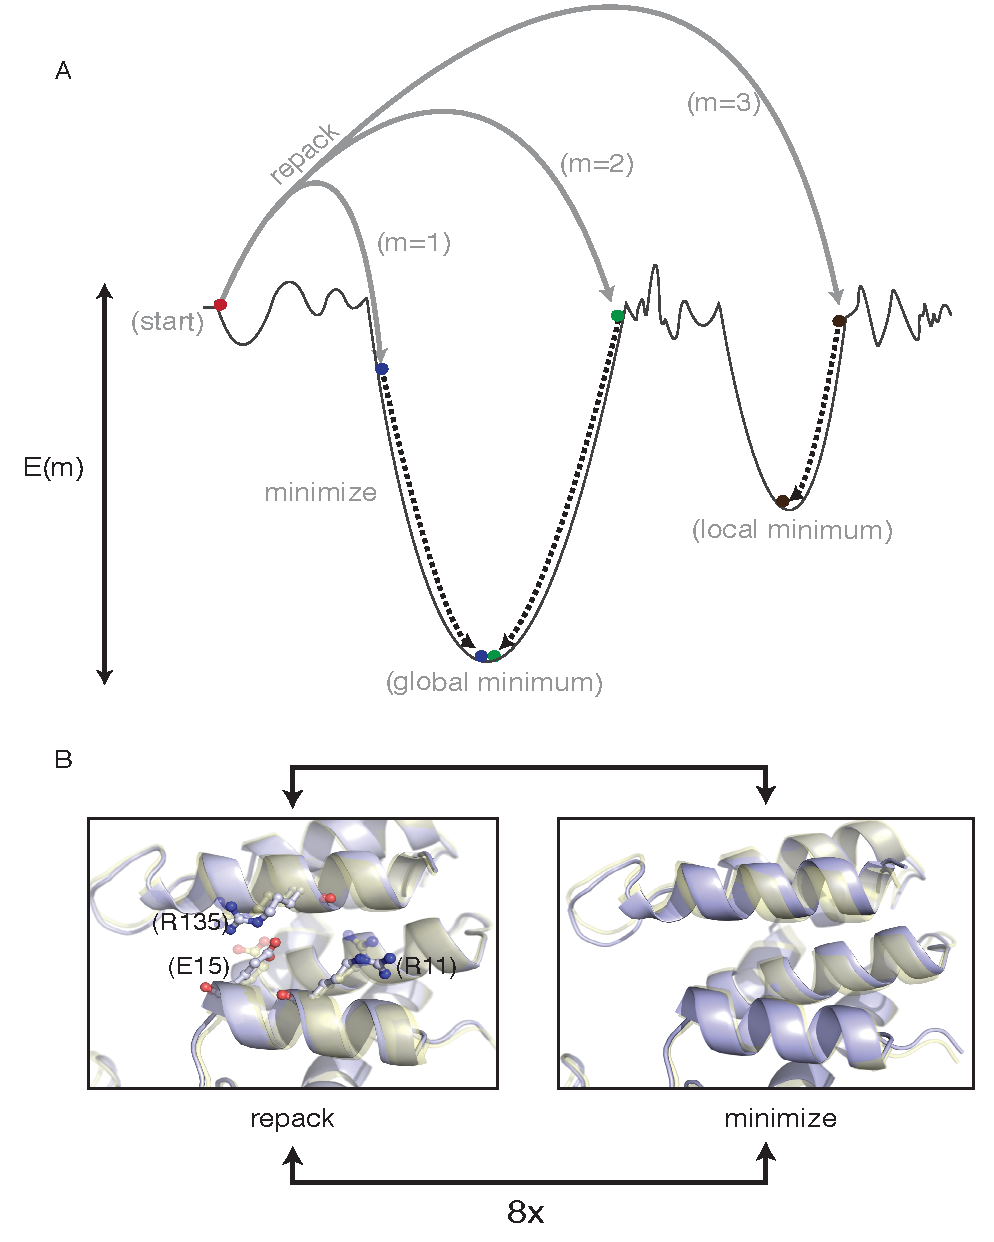
\includegraphics[scale=.7]{images/intro/figure1_9.pdf}
\caption[Refinement via Relax]{Refinement via Relax. Simplified energy landscape of a protein structure. The relax protocol combines small backbone perturbations with side-chain repacking. The coupling of Monte Carlo sampling with the Metropolis selection criterion allows for sampling of diverse conformations on the energy landscape. The final step is a gradient-based minimization of all torsion angles to move the model into the closest local energy minimum (A). Comparison of structural perturbations introduced by the repack and minimization steps. During repacking, the backbone of the input models fixed, whereas side-chain conformations from the rotamer library33 are sampled. Comparison of the initial (transparent yellow) and final (light blue) models reveals conservation of the R135 rotamer but changes to the R11 and E15 rotamers. Minimization affects all angles and changes the backbone conformation (B).}
\label{fig:minimization}
\end{figure}



\subsection{Rosetta Design}
Protein design, seeks to determine an amino acid sequence that folds into a given protein structure or performs a given function. The RosettaDesign algorithm is an iterative process that energetically optimizes both the structure and sequence of a protein \citep{Kuhlman:2003kp}. RosettaDesign alternates between rounds of fixed backbone sequence optimization and flexible backbone energy minimization. During the sequence optimization step, a Monte Carlo simulated annealing search is used to sample the sequence space. Every amino acid is considered at each position in the sequence, and rotamers are picked from to the Dunbrack library \citep{Dunbrack:1993jt}. After each round of Monte Carlo sequence optimization, the backbone is relaxed to accommodate the designed amino acids. The practical uses of RosettaDesign can be divided into five basic categories: design of novel folds. Redesign of existing proteins, design to enhance knowledge of structure, enzyme design, and design applied to translational medicine. 

\subsubsection{Design of Novel Folds}
The RosettaDesign method was implemented by Kuhlman and colleagues \citep{Kuhlman:2000tc}. The method has been used for the \textit{de novo} design of a fold that was not (yet) represented in the PDB \citep{Kuhlman:2003kp}. This was arguably the start of the "golden age" of protein design and gave credibility to the algorithm. A starting backbone model consisting of a five-strand $\beta$-sheet and two packed helices was constructed with the Rosetta \textit{de novo} protocol using distance constraints derived from a two-dimensional sketch. The sequence was iteratively designed with five simulation trials of 15 cycles each. The final sequence was expressed, and the structure was determined using X-ray crystallography. The experimental structure has a deviation to the predicted structure of <1.1 angstroms.

\subsubsection{Redesign of Existing Proteins}
When nine globular proteins were stripped of all side chains and then redesigned using RosettaDesign, the average sequence recovery was 35\% for all residues \citep{Dantas:2003vt}. In four of nine cases, the protein stability improved as measured by chemical denaturation. The structure of a redesigned human protein was determined experimentally.  RosettaDesign was then used to systematically identify mutations of carboxypeptidase that would improve the stability of the protein. All of the tested mutants were more stable than the wild-type protein, with the top-scoring mutant having a reduction of free energy of 5.2 kcal/mol.

\subsubsection{Design to Enhance Knowledge of Structure}
Protein design approaches have enhanced our knowledge of how protein sequence relates to protein structure. For instance, the finding that designed protein sequences are highly similar to the native sequence suggests that native protein sequences are optimal for their structure \citep{Kuhlman:2000tc}. Babor and Kortemme investigated the antibody sequence-structure relationship using RosettaDesign. They demonstrated that native sequences of antibody HCDR3 loops are optimal for conformational flexibility \citep{Babor:2009it}. The authors collected pairs of unbound and antigen-bound antibody structures. They used multiconstraint design to find low-scoring sequences that were consistent with both unbound and bound structures. The sequences predicted by multiconstraint design were more similar to the native sequences than the sequences predicted to preferentially bind either the unbound or bound conformations. 

\subsubsection{Enzyme Design}
The RosettaMatch algorithm starts from the protein backbone and attempts to build toward the specified transition state geometry \citep{Zanghellini:2006is}. In this method, all possible active site positions are defined for the protein scaffold, and rotamers from the Dunbrack library are placed at each sequence position in the catalytic site. The sequence of the area surrounding the catalytic site is then designed. 
Recently, the RosettaMatch algorithm was used to design enzymes that catalyze the retro-aldol reaction \citep{Jiang:2008jk}.The degrees of freedom in the transition state, the orientation of the active site side chains, and the conformations of the active site side chains were simultaneously optimized. Of 72 models tested, a total of 32 were found to have catalytic activity as much as four orders of magnitude greater than that of an uncatalyzed reaction. Two of the active enzymes were crystallized. The experimental structures share a high degree of similarity with the computational design although the loop regions surrounding the catalytic site show significant variance from the model.

Computationally designed functional Kemp elimination catalysts using RosettaMatch have also been designed. Quantum chemical predictions were used to generate an idealized transition state model, and RosettaMatch was used to search for backbone configurations that would support the predicted transition sate \citep{Rothlisberger:2008ef}. 

\subsubsection{Design Applied to Translational Medicine}
The successes of the RosettaDesign algorithm in predicting new sequences that optimize binding and answer questions about protein structure lead to its application to more bio-medical applications such as vaccine design and protein therapeutics. Fleishman et al. used the paratope of an antibody to find hotspot positions that neutralized influenza. Using these positions, they designed a protein that would properly present a mimic of the paratope. The crystal structure of the design indicated that it did indeed present mimicry while functional studies confirmed its neutralization capacity \citep{Fleishman:2011fx}.
The works of the Schief group have expanded design to explore novel scaffolding approaches to be used as immunogens. Using RosettaDesign, they presented the epitope to broadly neutralizing antibodies 2F5 and 4E10 to HIV which elicited this class of antibody in animal models \citep{Correia:2010ck,Ofek:2010bv}. In addition, they have used RosettaDesign to target potently neutralizing antibodies against the CD4 site while eliminated binding to non-neutralizing antibodies that bind to decoy epitopes \citep{Wu:2010jv}. More recently, this lab has used design to mimic an epitope to RSV that is now being tried in animal models \citep{Correia:2014jp}.

A current major challenge in protein design is the \textit{de novo} design of a novel protein-protein interface. So far, the most successful attempts at \textit{de novo} interface design have been relatively modest, focusing on small proteins and yielding micromolar affinity \citep{Mandell:2009he,Huang:2007ge}. This small boost affinity often requires display technology to increase potency and specificity. The Rosetta community is well aware of these limitations and work on increasing the accuracy of predicted interface mutations, particularly around hydrogen bonding networks and explicit solvent models \citep{Combs:2012tl}. 


